\documentclass[onesided]{article}\usepackage[]{graphicx}\usepackage[]{color}
% maxwidth is the original width if it is less than linewidth
% otherwise use linewidth (to make sure the graphics do not exceed the margin)
\makeatletter
\def\maxwidth{ %
  \ifdim\Gin@nat@width>\linewidth
    \linewidth
  \else
    \Gin@nat@width
  \fi
}
\makeatother

\definecolor{fgcolor}{rgb}{0.345, 0.345, 0.345}
\newcommand{\hlnum}[1]{\textcolor[rgb]{0.686,0.059,0.569}{#1}}%
\newcommand{\hlstr}[1]{\textcolor[rgb]{0.192,0.494,0.8}{#1}}%
\newcommand{\hlcom}[1]{\textcolor[rgb]{0.678,0.584,0.686}{\textit{#1}}}%
\newcommand{\hlopt}[1]{\textcolor[rgb]{0,0,0}{#1}}%
\newcommand{\hlstd}[1]{\textcolor[rgb]{0.345,0.345,0.345}{#1}}%
\newcommand{\hlkwa}[1]{\textcolor[rgb]{0.161,0.373,0.58}{\textbf{#1}}}%
\newcommand{\hlkwb}[1]{\textcolor[rgb]{0.69,0.353,0.396}{#1}}%
\newcommand{\hlkwc}[1]{\textcolor[rgb]{0.333,0.667,0.333}{#1}}%
\newcommand{\hlkwd}[1]{\textcolor[rgb]{0.737,0.353,0.396}{\textbf{#1}}}%
\let\hlipl\hlkwb

\usepackage{framed}
\makeatletter
\newenvironment{kframe}{%
 \def\at@end@of@kframe{}%
 \ifinner\ifhmode%
  \def\at@end@of@kframe{\end{minipage}}%
  \begin{minipage}{\columnwidth}%
 \fi\fi%
 \def\FrameCommand##1{\hskip\@totalleftmargin \hskip-\fboxsep
 \colorbox{shadecolor}{##1}\hskip-\fboxsep
     % There is no \\@totalrightmargin, so:
     \hskip-\linewidth \hskip-\@totalleftmargin \hskip\columnwidth}%
 \MakeFramed {\advance\hsize-\width
   \@totalleftmargin\z@ \linewidth\hsize
   \@setminipage}}%
 {\par\unskip\endMakeFramed%
 \at@end@of@kframe}
\makeatother

\definecolor{shadecolor}{rgb}{.97, .97, .97}
\definecolor{messagecolor}{rgb}{0, 0, 0}
\definecolor{warningcolor}{rgb}{1, 0, 1}
\definecolor{errorcolor}{rgb}{1, 0, 0}
\newenvironment{knitrout}{}{} % an empty environment to be redefined in TeX

\usepackage{alltt}
\usepackage[T1]{fontenc}
\linespread{1.5} % Line spacing - Palatino needs more space between lines
\usepackage{microtype} % Slightly tweak font spacing for aesthetics

\usepackage[hmarginratio=1:1,columnsep=20pt]{geometry} % Document margins
%\usepackage{multicol} % Used for the two-column layout of the document
\usepackage[hang, small,labelfont=bf,up,textfont=it,up]{caption} % Custom captions under/above floats in tables or figures
\usepackage{booktabs} % Horizontal rules in tables
\usepackage{float} % Required for tables and figures in the multi-column environment - they need to be placed in specific locations with the [H] (e.g. \begin{table}[H])

\usepackage{lettrine} % The lettrine is the first enlarged letter at the beginning of the text
\usepackage{paralist} % Used for the compactitem environment which makes bullet points with less space between them

% to ignore texts: good for thank messages and paper submissions.
      % \fbox{\phantom{This text will be invisible too, but a box will be printed arround it.}}

\usepackage{abstract} % Allows abstract customization
\renewcommand{\abstractnamefont}{\normalfont\bfseries} % Set the "Abstract" text to bold
%\renewcommand{\abstracttextfont}{\normalfont\small\itshape} % Set the abstract itself to small italic text

\usepackage[]{titlesec} % Allows customization of titles
\renewcommand\thesection{\Roman{section}} % Roman numerals for the sections
\renewcommand\thesubsection{\Roman{subsection}} % Roman numerals for subsections
\titleformat{\section}[block]{\large\scshape\centering}{\thesection.}{1em}{} % Change the look of the section titles
\titleformat{\subsection}[block]{\large}{\thesubsection.}{1em}{} % Change the look of the section titles

\usepackage{fancybox, fancyvrb, calc}
\usepackage[svgnames]{xcolor}
\usepackage{epigraph}
\usepackage{longtable}
\usepackage{pdflscape}
\usepackage{graphics}
\usepackage{pbox} % \pbox{20cm}{This is the first \\ cell}
\usepackage{amsfonts}
\usepackage{amsmath}
\usepackage{amssymb}
\usepackage{rotating}
\usepackage{paracol}
\usepackage{textcomp}
\usepackage[export]{adjustbox}
\usepackage{afterpage}
\usepackage{filecontents}
\usepackage{color}
\usepackage{latexsym}
\usepackage{lscape}       %\begin{landscape} and \end{landscape}
\usepackage{wasysym}
\usepackage{dashrule}

\usepackage{framed}
\usepackage{tree-dvips}
\usepackage{pgffor}
\usepackage[]{authblk}
\usepackage{setspace}
\usepackage{array}
\usepackage[latin1]{inputenc}
\usepackage{hyperref}     %desactivar para link rojos
\usepackage{graphicx}
\usepackage{dcolumn} % for R tables
\usepackage{multirow} % For multirow in tables
\usepackage{pifont}
\usepackage{listings}




% hypothesis / theorem package begin
\usepackage{amsthm}
\usepackage{thmtools}
\declaretheoremstyle[
spaceabove=6pt, spacebelow=6pt,
headfont=\normalfont\bfseries,
notefont=\mdseries, notebraces={(}{)},
bodyfont=\normalfont,
postheadspace=0.6em,
headpunct=:
]{mystyle}
\declaretheorem[style=mystyle, name=Hypothesis, preheadhook={\renewcommand{\thehyp}{H\textsubscript{\arabic{hyp}}}}]{hyp}

\usepackage{cleveref}
\crefname{hyp}{hypothesis}{hypotheses}
\Crefname{hyp}{Hypothesis}{Hypotheses}
% hypothesis / theorem package end


%----------------------------------------------------------------------------------------
% Other ADDS-ON
%----------------------------------------------------------------------------------------

% independence symbol \independent
\newcommand\independent{\protect\mathpalette{\protect\independenT}{\perp}}
\def\independenT#1#2{\mathrel{\rlap{$#1#2$}\mkern2mu{#1#2}}}







\hypersetup{
    bookmarks=true,         % show bookmarks bar?
    unicode=false,          % non-Latin characters in Acrobat's bookmarks
    pdftoolbar=true,        % show Acrobat's toolbar?
    pdfmenubar=true,        % show Acrobat's menu?
    pdffitwindow=true,     % window fit to page when opened
    pdfstartview={FitH},    % fits the width of the page to the window
    pdftitle={My title},    % title
    pdfauthor={Author},     % author
    pdfsubject={Subject},   % subject of the document
    pdfcreator={Creator},   % creator of the document
    pdfproducer={Producer}, % producer of the document
    pdfkeywords={keyword1} {key2} {key3}, % list of keywords
    pdfnewwindow=true,      % links in new window
    colorlinks=true,       % false: boxed links; true: colored links
    linkcolor=ForestGreen,          % color of internal links (change box color with linkbordercolor)
    citecolor=ForestGreen,        % color of links to bibliography
    filecolor=ForestGreen,      % color of file links
    urlcolor=ForestGreen           % color of external links
}

%\usepackage[nodayofweek,level]{datetime} % to have date within text

\newcommand{\LETT}[3][]{\lettrine[lines=4,loversize=.2,#1]{\smash{#2}}{#3}} % letrine customization



% comments on margin
  % Select what to do with todonotes: 
  % \usepackage[disable]{todonotes} % notes not showed
  \usepackage[draft]{todonotes}   % notes showed
  % usage: \todo{This is a note at margin}

\usepackage{cooltooltips}

%%% bib begin
\usepackage[american]{babel}
\usepackage{csquotes}
\usepackage[backend=biber,style=authoryear,dashed=false,doi=false,isbn=false,url=false,arxiv=false]{biblatex}
%\DeclareLanguageMapping{american}{american-apa}
\addbibresource{/Users/hectorbahamonde/Bibliografia_PoliSci/library.bib} 
\addbibresource{/Users/hectorbahamonde/Bibliografia_PoliSci/Bahamonde_BibTex2013.bib} 

% USAGES
%% use \textcite to cite normal
%% \parencite to cite in parentheses
%% \footcite to cite in footnote
%% the default can be modified in autocite=FOO, footnote, for ex. 
%%% bib end

\usepackage{fancyhdr} % Headers and footers
\pagestyle{fancy} % All pages have headers and footers
\fancyhead{} % Blank out the default header
\fancyfoot{} % Blank out the default footer
\fancyhead[C]{Incorporando el Elemento Tiempo: Fixed effects y Differences-in-Differences} % Custom header text
\fancyfoot[RO,LE]{\thepage} % Custom footer text
\IfFileExists{upquote.sty}{\usepackage{upquote}}{}
\begin{document}
% DOCUMENT ID
%----------------------------------------------------------------------------------------
%	CONTENT
%----------------------------------------------------------------------------------------

%\graphicspath{
%{/Users/hectorbahamonde/RU/Term5/Experiments_Redlawsk/Experiment/Data/}
%}



%%%%%%%%%%%%%%%%%%%%%%%%%%%%%%%%%%%%%%%%%%%%%%


%%%%%%%%%%%%%%%%%%%%%%%%%%%%%%%%%%%%%%%%%%%%%%





\hspace{-5mm}{\bf Profesor}: H\'ector Bahamonde, PhD.\\
\texttt{e:}\href{mailto:hector.bahamonde@uoh.cl}{\texttt{hector.bahamonde@uoh.cl}}\\
\texttt{w:}\href{http://www.hectorbahamonde.com}{\texttt{www.hectorbahamonde.com}}\\
{\bf Curso}: MLE.\\
\hspace{-5mm}{\bf TA}: Gonzalo Barr\'ia.

\section{Introducci\'on}

Algunas veces tenemos la oportunidad de construir un contrafactual donde tanto $i_{\tau(1)}$ como $i_{\tau(0)}$ son observados para el \emph{mismo} $i$. Esto en general sucede cuando observamos a $i$ en dos tiempos distintos, esto es, en $i_{t}$ y $i_{t+1}$, o en f\'acil, $i$ \emph{antes} de que se le administre $\tau$ e $i$ \emph{despu\'es} de que se le administre $\tau$. En este tipo de casos estar\'iamos en posici\'on de ver ambos ``universos paralelos''. Cuando tenemos los mismos $i$'s repetidos en el tiempo, solemos llamar a esta estructura de datos ``panel data''. Esto se debe a que cada $i$ es un ``panel'' que se repite, en este ejemplo, dos veces ($t_{1}$ y $t_{2}$). Pueden ser m\'as veces en todo caso.

Sin embargo, esto no viene sin problemas. Hoy veremos dos t\'ecnicas:

\begin{enumerate}
  \item \emph{Fixed effects}.
  \item \emph{Difference in Differences}.
\end{enumerate}

y ambas trabajan con ``panel data''. Veamos c\'omo se ven los datos de panel:

\begin{knitrout}
\definecolor{shadecolor}{rgb}{0.969, 0.969, 0.969}\color{fgcolor}\begin{kframe}
\begin{alltt}
\hlkwd{p_load}\hlstd{(AER, plm, stargazer)}
\hlkwd{data}\hlstd{(Fatalities)}
\hlkwd{head}\hlstd{(Fatalities)[}\hlnum{1}\hlopt{:}\hlnum{2}\hlstd{]}
\end{alltt}
\begin{verbatim}
##   state year
## 1    al 1982
## 2    al 1983
## 3    al 1984
## 4    al 1985
## 5    al 1986
## 6    al 1987
\end{verbatim}
\end{kframe}
\end{knitrout}



\section{Fixed Effects}

Una de las ventajas de la randomizaci\'on es que ``borra'' (o ``ignora'') las caracter\'isticas (observables y no) de $i$ y asigna el tratamiento $\tau$ independientemente de esas caracter\'isticas (esta es el ``\emph{ignorability assumption}''). Sin embargo, en el mundo observacional (i.e. no experimental) esto no es posible. Qu\'e herramientas podemos en el mundo observacional para tratar de aproximarnos al mundo experimental y ``borrar'' las caracter\'isticas individuales de todos los $i$? Recuerda que si los $i$'s son similares, podemos atribuir el efecto causal observado s\'olo a la administraci\'on de $\tau$. Al ``neutralizar'' la caracter\'isticas individuales de cada $i$, los \emph{fixed effects} hacen justamente eso. 

Supongamos que necesitamos estimar 

\begin{equation}\label{fe}
\alpha
\end{equation}


\section{Difference in Differences}

Otra herramienta que podemos usar cuando se trata de trabajar con tiempo, es el \emph{difference in differences}. \textcite{Card1994} tratan de usar la geograf\'ia como \emph{as-if random} factor ({\color{red}?}). La pregunta que ellos ten\'ian era cu\'al es el efecto (causal?) en el empleo ante un incremento en el salario en el sector de comida r\'apida. En otras palabras, \emph{qu\'e ocurre con el empleo en este sector cuando aumenta el salario, sube o baja?}


\begin{knitrout}
\definecolor{shadecolor}{rgb}{0.969, 0.969, 0.969}\color{fgcolor}\begin{kframe}
\begin{alltt}
\hlcom{# instalar librerias}
\hlkwd{p_load}\hlstd{(ggplot2,dplyr,maps)}
\hlcom{# declarar datos}
\hlstd{all_states} \hlkwb{<-} \hlkwd{map_data}\hlstd{(}\hlstr{"state"}\hlstd{)}
\hlcom{# plot}
\hlkwd{ggplot}\hlstd{(all_states,}
       \hlkwd{aes}\hlstd{(}\hlkwc{x}\hlstd{=long,} \hlkwc{y}\hlstd{=lat,} \hlkwc{group} \hlstd{= group))} \hlopt{+}
  \hlkwd{geom_polygon}\hlstd{(}\hlkwc{fill}\hlstd{=}\hlstr{"grey"}\hlstd{,} \hlkwc{colour} \hlstd{=} \hlstr{"white"}\hlstd{)} \hlopt{+}
  \hlkwd{geom_polygon}\hlstd{(}\hlkwc{fill}\hlstd{=}\hlstr{"green"}\hlstd{,} \hlkwc{data} \hlstd{=} \hlkwd{filter}\hlstd{(all_states, region} \hlopt \hlkwd{c}\hlstd{(}\hlstr{"pennsylvania"}\hlstd{)))} \hlopt{+}
  \hlkwd{geom_polygon}\hlstd{(}\hlkwc{fill}\hlstd{=}\hlstr{"red"}\hlstd{,} \hlkwc{data} \hlstd{=} \hlkwd{filter}\hlstd{(all_states, region} \hlopt \hlkwd{c}\hlstd{(}\hlstr{"new jersey"}\hlstd{))}
               \hlstd{)} \hlopt{+}
  \hlkwd{theme_bw}\hlstd{()} \hlopt{+}
  \hlkwd{xlab}\hlstd{(}\hlstr{"Longitud"}\hlstd{)} \hlopt{+}
  \hlkwd{ylab}\hlstd{(}\hlstr{"Latitud"}\hlstd{)}
\end{alltt}
\end{kframe}

{\centering 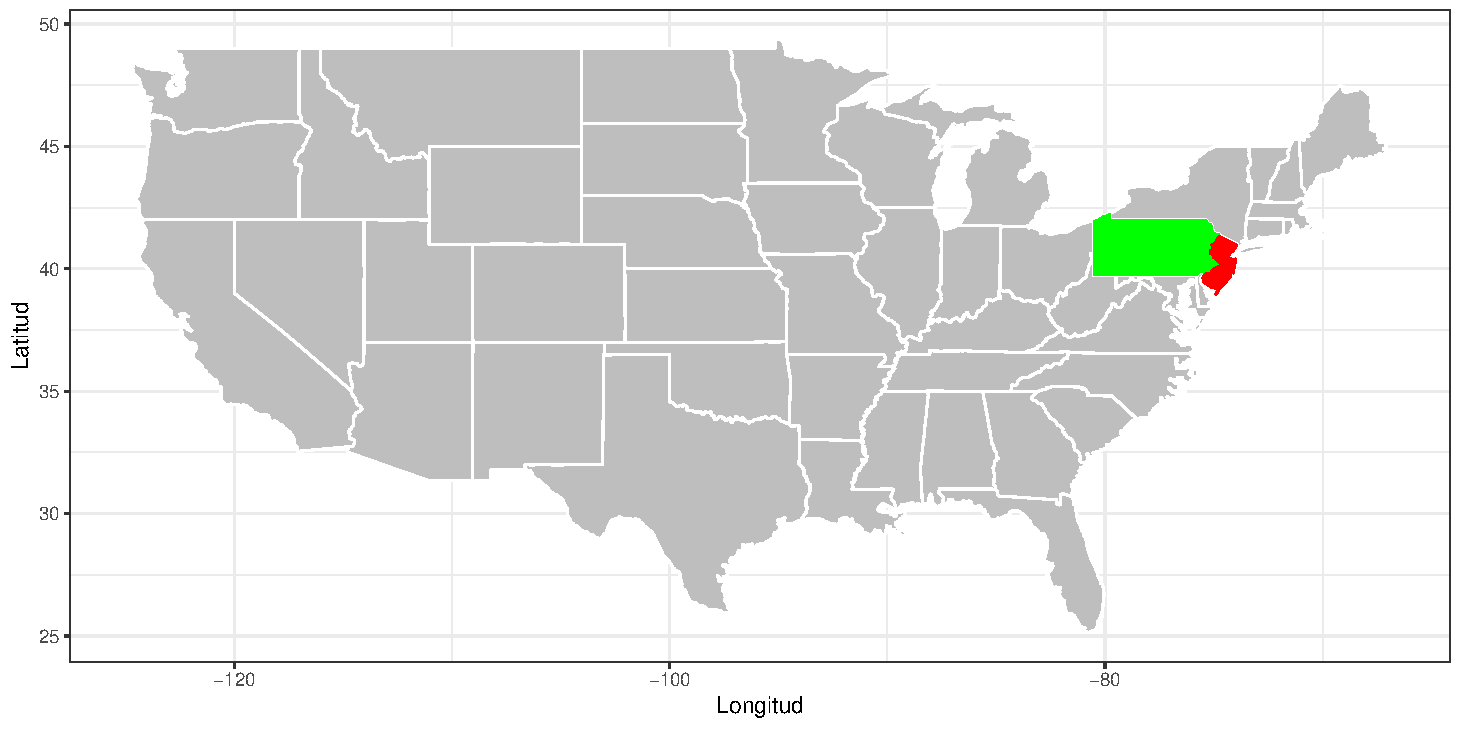
\includegraphics[width=\maxwidth]{figure/us:map-1} 

}



\end{knitrout}

Sin embargo, PA y NJ puede que hayan sido distintos en varias caracter\'isticas (que es lo m\'as probable, no?). El problema es que si quisi\'eramos calcular el efecto causal Desempleo$_{\text{PA}}$-Desempleo$_{\text{NJ}}$ cuando subimos el salario en NJ, ya PA podr\'ia contar con un piso que no estemos tomando en consideraci\'on. C\'omo podr\'iamos calcular el efecto causal $\tau$, pero \emph{tomando en cuenta las caracter\'isticas de base de PA}?

Ve\'amos un gr\'afico que podr\'ia aclarar lo que queremos.

\begin{knitrout}
\definecolor{shadecolor}{rgb}{0.969, 0.969, 0.969}\color{fgcolor}\begin{kframe}
\begin{alltt}
\hlkwd{plot}\hlstd{(}\hlkwd{c}\hlstd{(}\hlnum{0}\hlstd{,} \hlnum{1}\hlstd{),} \hlkwd{c}\hlstd{(}\hlnum{6}\hlstd{,} \hlnum{8}\hlstd{),}
     \hlkwc{type} \hlstd{=} \hlstr{"p"}\hlstd{,}
     \hlkwc{ylim} \hlstd{=} \hlkwd{c}\hlstd{(}\hlnum{5}\hlstd{,} \hlnum{12}\hlstd{),}
     \hlkwc{xlim} \hlstd{=} \hlkwd{c}\hlstd{(}\hlopt{-}\hlnum{0.3}\hlstd{,} \hlnum{1.3}\hlstd{),}
     \hlkwc{main} \hlstd{=} \hlstr{"El Estimador de Difference in Difference"}\hlstd{,}
     \hlkwc{xlab} \hlstd{=} \hlstr{"Periodo"}\hlstd{,}
     \hlkwc{ylab} \hlstd{=} \hlstr{"Desempleo"}\hlstd{,}
     \hlkwc{col} \hlstd{=} \hlstr{"steelblue"}\hlstd{,}
     \hlkwc{pch} \hlstd{=} \hlnum{20}\hlstd{,}
     \hlkwc{xaxt} \hlstd{=} \hlstr{"n"}\hlstd{,}
     \hlkwc{yaxt} \hlstd{=} \hlstr{"n"}\hlstd{)}
\hlcom{#}
\hlkwd{axis}\hlstd{(}\hlnum{1}\hlstd{,} \hlkwc{at} \hlstd{=} \hlkwd{c}\hlstd{(}\hlnum{0}\hlstd{,} \hlnum{1}\hlstd{),} \hlkwc{labels} \hlstd{=} \hlkwd{c}\hlstd{(}\hlstr{"Antes"}\hlstd{,} \hlstr{"Despues"}\hlstd{))}
\hlkwd{axis}\hlstd{(}\hlnum{2}\hlstd{,} \hlkwc{at} \hlstd{=} \hlkwd{c}\hlstd{(}\hlnum{0}\hlstd{,} \hlnum{13}\hlstd{))}
\hlcom{# treatment}
\hlkwd{points}\hlstd{(}\hlkwd{c}\hlstd{(}\hlnum{0}\hlstd{,} \hlnum{1}\hlstd{,} \hlnum{1}\hlstd{),} \hlkwd{c}\hlstd{(}\hlnum{7}\hlstd{,} \hlnum{9}\hlstd{,} \hlnum{11}\hlstd{),}
       \hlkwc{col} \hlstd{=} \hlstr{"darkred"}\hlstd{,}
       \hlkwc{pch} \hlstd{=} \hlnum{20}\hlstd{)}
\hlcom{# }
\hlkwd{lines}\hlstd{(}\hlkwd{c}\hlstd{(}\hlnum{0}\hlstd{,} \hlnum{1}\hlstd{),} \hlkwd{c}\hlstd{(}\hlnum{7}\hlstd{,} \hlnum{11}\hlstd{),} \hlkwc{col} \hlstd{=} \hlstr{"darkred"}\hlstd{)}
\hlkwd{lines}\hlstd{(}\hlkwd{c}\hlstd{(}\hlnum{0}\hlstd{,} \hlnum{1}\hlstd{),} \hlkwd{c}\hlstd{(}\hlnum{6}\hlstd{,} \hlnum{8}\hlstd{),} \hlkwc{col} \hlstd{=} \hlstr{"steelblue"}\hlstd{)}
\hlkwd{lines}\hlstd{(}\hlkwd{c}\hlstd{(}\hlnum{0}\hlstd{,} \hlnum{1}\hlstd{),} \hlkwd{c}\hlstd{(}\hlnum{7}\hlstd{,} \hlnum{9}\hlstd{),} \hlkwc{col} \hlstd{=} \hlstr{"darkred"}\hlstd{,} \hlkwc{lty} \hlstd{=} \hlnum{2}\hlstd{)}
\hlkwd{lines}\hlstd{(}\hlkwd{c}\hlstd{(}\hlnum{1}\hlstd{,} \hlnum{1}\hlstd{),} \hlkwd{c}\hlstd{(}\hlnum{9}\hlstd{,} \hlnum{11}\hlstd{),} \hlkwc{col} \hlstd{=} \hlstr{"black"}\hlstd{,} \hlkwc{lty} \hlstd{=} \hlnum{2}\hlstd{,} \hlkwc{lwd} \hlstd{=} \hlnum{2}\hlstd{)}
\hlcom{# }
\hlkwd{text}\hlstd{(}\hlnum{1}\hlstd{,} \hlnum{10}\hlstd{,} \hlkwd{expression}\hlstd{(tau),} \hlkwc{cex} \hlstd{=} \hlnum{0.8}\hlstd{,} \hlkwc{pos} \hlstd{=} \hlnum{4}\hlstd{)}
\hlkwd{text}\hlstd{(}\hlnum{0}\hlstd{,} \hlnum{5.5}\hlstd{,} \hlstr{"Control antes (PA)"}\hlstd{,} \hlkwc{cex} \hlstd{=} \hlnum{0.8} \hlstd{,} \hlkwc{pos} \hlstd{=} \hlnum{4}\hlstd{)}
\hlkwd{text}\hlstd{(}\hlnum{0}\hlstd{,} \hlnum{6.8}\hlstd{,} \hlstr{"Treated antes (NJ)"}\hlstd{,} \hlkwc{cex} \hlstd{=} \hlnum{0.8} \hlstd{,} \hlkwc{pos} \hlstd{=} \hlnum{4}\hlstd{)}
\hlkwd{text}\hlstd{(}\hlnum{1}\hlstd{,} \hlnum{7.9}\hlstd{,} \hlstr{"Control despues (PA)"}\hlstd{,} \hlkwc{cex} \hlstd{=} \hlnum{0.8} \hlstd{,} \hlkwc{pos} \hlstd{=} \hlnum{4}\hlstd{)}
\hlkwd{text}\hlstd{(}\hlnum{1}\hlstd{,} \hlnum{11.1}\hlstd{,} \hlstr{"Treated despues (NJ)"}\hlstd{,} \hlkwc{cex} \hlstd{=} \hlnum{0.8} \hlstd{,} \hlkwc{pos} \hlstd{=} \hlnum{4}\hlstd{)}
\end{alltt}
\end{kframe}

{\centering 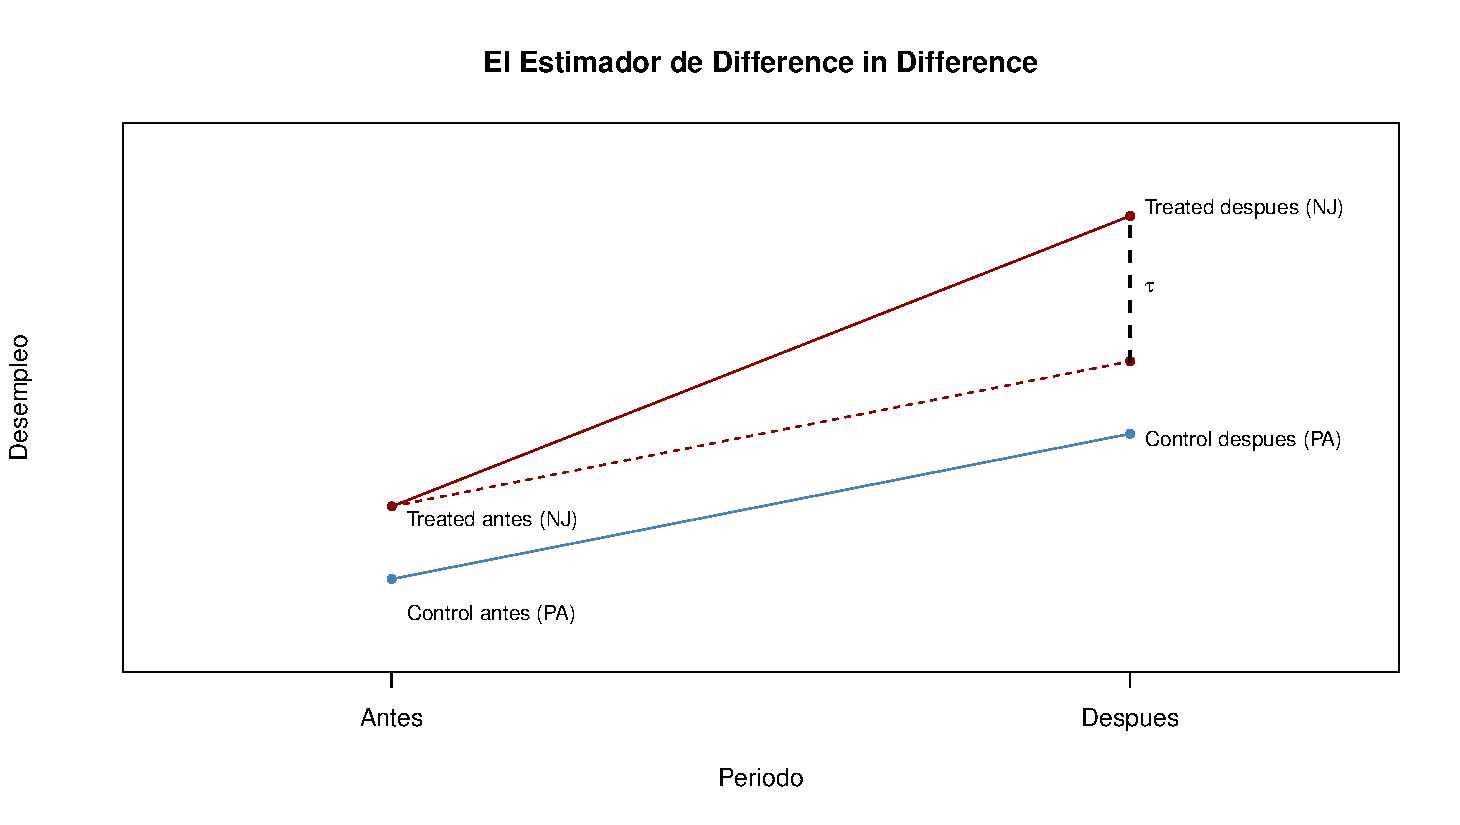
\includegraphics[width=\maxwidth]{figure/dif:dif-1} 

}



\end{knitrout}

\begin{itemize}
\item {\color{red}Cu\'al es el contrafactual?}
\item {\color{red}Qu\'e significa o c\'omo leemos $\tau$?}
\end{itemize}


De manera m\'as formal, $\tau=\beta_{1}$ en \autoref{ols}:

\begin{equation}\label{ols}
\Delta y_{i} = \beta_{0} + \beta_{1}z_{i} + \epsilon_{i}
\end{equation}

donde $z$ es el \emph{estado} del tratamiento, b\'asicamente un vector $x$ de 0's y 1's, $\Delta y_{i}$ es la diferencia (el ``delta'') en $y$ cuando $z(0)$ cambia a $z(1)$, y $\tau=\beta_{1}$ es el \emph{DID estimator} especificado en \autoref{did}:


\begin{equation}\label{did}
\tau = (y_{\text{Control Antes}}-y_{\text{Control Despu\'es}}) - (y_{\text{Treated Antes}}-y_{\text{Treated Despu\'es}})
\end{equation}

Si te fijas, el estimador es ``la diferencia de la diferencia'' (o ``\emph{difference in difference}'').


Cocinemos unos datos.

\begin{knitrout}
\definecolor{shadecolor}{rgb}{0.969, 0.969, 0.969}\color{fgcolor}\begin{kframe}
\begin{alltt}
\hlstd{n} \hlkwb{<-} \hlnum{200}
\hlcom{# definir tau}
\hlstd{TEffect} \hlkwb{<-} \hlnum{4}
\hlcom{# generar dummy de treatment }
\hlstd{z} \hlkwb{<-} \hlkwd{c}\hlstd{(}\hlkwd{rep}\hlstd{(}\hlnum{0}\hlstd{, n}\hlopt{/}\hlnum{2}\hlstd{),} \hlkwd{rep}\hlstd{(}\hlnum{1}\hlstd{, n}\hlopt{/}\hlnum{2}\hlstd{))}
\hlcom{# simular pre y post treatment en la y}
\hlstd{y_pre} \hlkwb{<-} \hlnum{7} \hlopt{+} \hlkwd{rnorm}\hlstd{(n)}
\hlstd{y_pre[}\hlnum{1}\hlopt{:}\hlstd{n}\hlopt{/}\hlnum{2}\hlstd{]} \hlkwb{<-} \hlstd{y_pre[}\hlnum{1}\hlopt{:}\hlstd{n}\hlopt{/}\hlnum{2}\hlstd{]} \hlopt{-} \hlnum{1}
\hlstd{y_post} \hlkwb{<-} \hlnum{7} \hlopt{+} \hlnum{2} \hlopt{+} \hlstd{TEffect} \hlopt{*} \hlstd{z} \hlopt{+} \hlkwd{rnorm}\hlstd{(n)}
\hlstd{y_post[}\hlnum{1}\hlopt{:}\hlstd{n}\hlopt{/}\hlnum{2}\hlstd{]} \hlkwb{<-} \hlstd{y_post[}\hlnum{1}\hlopt{:}\hlstd{n}\hlopt{/}\hlnum{2}\hlstd{]} \hlopt{-} \hlnum{1}
\hlcom{#}
\hlkwd{p_load}\hlstd{(scales)} \hlcom{# para usar alpha abajo (colores)}
\hlstd{pre} \hlkwb{<-} \hlkwd{rep}\hlstd{(}\hlnum{0}\hlstd{,} \hlkwd{length}\hlstd{(y_pre[z}\hlopt{==}\hlnum{0}\hlstd{]))}
\hlstd{post} \hlkwb{<-} \hlkwd{rep}\hlstd{(}\hlnum{1}\hlstd{,} \hlkwd{length}\hlstd{(y_pre[z}\hlopt{==}\hlnum{0}\hlstd{]))}
\hlcom{# t=1}
\hlkwd{plot}\hlstd{(}\hlkwd{jitter}\hlstd{(pre,} \hlnum{0.6}\hlstd{),}
     \hlstd{y_pre[z} \hlopt{==} \hlnum{0}\hlstd{],}
     \hlkwc{ylim} \hlstd{=} \hlkwd{c}\hlstd{(}\hlnum{0}\hlstd{,} \hlnum{16}\hlstd{),}
     \hlkwc{col} \hlstd{=} \hlkwd{alpha}\hlstd{(}\hlstr{"steelblue"}\hlstd{,} \hlnum{0.3}\hlstd{),}
     \hlkwc{pch} \hlstd{=} \hlnum{20}\hlstd{,}
     \hlkwc{xlim} \hlstd{=} \hlkwd{c}\hlstd{(}\hlopt{-}\hlnum{0.5}\hlstd{,} \hlnum{1.5}\hlstd{),}
     \hlkwc{ylab} \hlstd{=} \hlstr{"Y"}\hlstd{,}
     \hlkwc{xlab} \hlstd{=} \hlstr{"Periodo"}\hlstd{,}
     \hlkwc{xaxt} \hlstd{=} \hlstr{"n"}\hlstd{,}
     \hlkwc{main} \hlstd{=} \hlstr{"Simulacion del DID Estimator"}\hlstd{)}
\hlkwd{axis}\hlstd{(}\hlnum{1}\hlstd{,} \hlkwc{at} \hlstd{=} \hlkwd{c}\hlstd{(}\hlnum{0}\hlstd{,} \hlnum{1}\hlstd{),} \hlkwc{labels} \hlstd{=} \hlkwd{c}\hlstd{(}\hlstr{"Antes"}\hlstd{,} \hlstr{"Despues"}\hlstd{))}
\hlcom{# treatment t=1}
\hlkwd{points}\hlstd{(}\hlkwd{jitter}\hlstd{(pre,} \hlnum{0.6}\hlstd{),}
       \hlstd{y_pre[z} \hlopt{==} \hlnum{1}\hlstd{],}
       \hlkwc{col} \hlstd{=} \hlkwd{alpha}\hlstd{(}\hlstr{"darkred"}\hlstd{,} \hlnum{0.3}\hlstd{),}
       \hlkwc{pch} \hlstd{=} \hlnum{20}\hlstd{)}
\hlcom{# control t=2}
\hlkwd{points}\hlstd{(}\hlkwd{jitter}\hlstd{(post,} \hlnum{0.6}\hlstd{),}
       \hlstd{y_post[z} \hlopt{==} \hlnum{0}\hlstd{],}
       \hlkwc{col} \hlstd{=} \hlkwd{alpha}\hlstd{(}\hlstr{"steelblue"}\hlstd{,} \hlnum{0.5}\hlstd{),}
       \hlkwc{pch} \hlstd{=} \hlnum{20}\hlstd{)}
\hlcom{# treatment t=2}
\hlkwd{points}\hlstd{(}\hlkwd{jitter}\hlstd{(post,} \hlnum{0.6}\hlstd{),}
       \hlstd{y_post[z} \hlopt{==} \hlnum{1}\hlstd{],}
       \hlkwc{col} \hlstd{=} \hlkwd{alpha}\hlstd{(}\hlstr{"darkred"}\hlstd{,} \hlnum{0.5}\hlstd{),}
       \hlkwc{pch} \hlstd{=} \hlnum{20}\hlstd{)}
\hlcom{# lineas}
\hlkwd{lines}\hlstd{(}\hlkwd{c}\hlstd{(}\hlnum{0}\hlstd{,} \hlnum{1}\hlstd{),} \hlkwd{c}\hlstd{(}\hlkwd{mean}\hlstd{(y_pre[z} \hlopt{==} \hlnum{1}\hlstd{]),} \hlkwd{mean}\hlstd{(y_post[z} \hlopt{==} \hlnum{1}\hlstd{])),} \hlkwc{col} \hlstd{=} \hlstr{"darkred"}\hlstd{)}
\hlkwd{lines}\hlstd{(}\hlkwd{c}\hlstd{(}\hlnum{0}\hlstd{,} \hlnum{1}\hlstd{),} \hlkwd{c}\hlstd{(}\hlkwd{mean}\hlstd{(y_pre[z} \hlopt{==} \hlnum{0}\hlstd{]),} \hlkwd{mean}\hlstd{(y_post[z} \hlopt{==} \hlnum{0}\hlstd{])),} \hlkwc{col} \hlstd{=} \hlstr{"steelblue"}\hlstd{)}
\hlkwd{lines}\hlstd{(}\hlkwd{c}\hlstd{(}\hlnum{0}\hlstd{,} \hlnum{1}\hlstd{),} \hlkwd{c}\hlstd{(}\hlkwd{mean}\hlstd{(y_pre[z} \hlopt{==} \hlnum{1}\hlstd{]),} \hlkwd{mean}\hlstd{(y_post[z} \hlopt{==} \hlnum{0}\hlstd{])} \hlopt{+}
\hlstd{(}\hlkwd{mean}\hlstd{(y_pre[z} \hlopt{==} \hlnum{1}\hlstd{])}\hlopt{-}\hlkwd{mean}\hlstd{(y_pre[z} \hlopt{==} \hlnum{0}\hlstd{]))),} \hlkwc{col} \hlstd{=} \hlstr{"darkred"}\hlstd{,} \hlkwc{lty} \hlstd{=} \hlnum{2}\hlstd{)}
\end{alltt}
\end{kframe}

{\centering 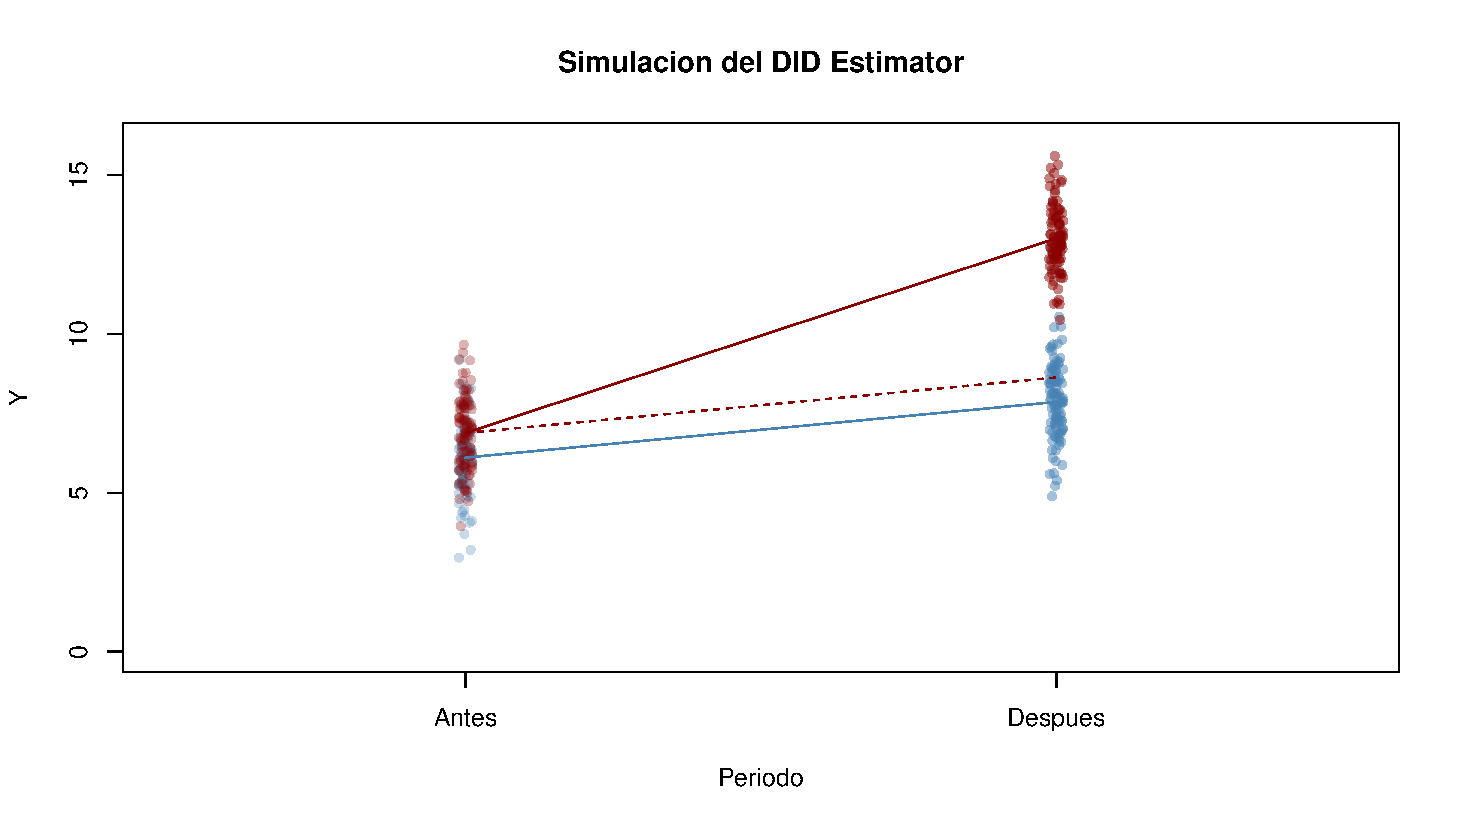
\includegraphics[width=\maxwidth]{figure/dif:dif:Data-1} 

}



\end{knitrout}

Ahora calculemos $\tau$ a mano:

\begin{knitrout}
\definecolor{shadecolor}{rgb}{0.969, 0.969, 0.969}\color{fgcolor}\begin{kframe}
\begin{alltt}
\hlkwd{mean}\hlstd{(y_post[z} \hlopt{==} \hlnum{1}\hlstd{])} \hlopt{-} \hlkwd{mean}\hlstd{(y_pre[z} \hlopt{==} \hlnum{1}\hlstd{])} \hlopt{-}
\hlstd{(}\hlkwd{mean}\hlstd{(y_post[z} \hlopt{==} \hlnum{0}\hlstd{])} \hlopt{-} \hlkwd{mean}\hlstd{(y_pre[z} \hlopt{==} \hlnum{0}\hlstd{]))}
\end{alltt}
\begin{verbatim}
## [1] 4.371355
\end{verbatim}
\end{kframe}
\end{knitrout}

Tambi\'en podemos usar \autoref{ols} para calcular $\tau$ (que recuerda es igual a $\beta_{1}$):

\begin{knitrout}
\definecolor{shadecolor}{rgb}{0.969, 0.969, 0.969}\color{fgcolor}\begin{kframe}
\begin{alltt}
\hlkwd{lm}\hlstd{(}\hlkwd{I}\hlstd{(y_post} \hlopt{-} \hlstd{y_pre)} \hlopt{~} \hlstd{z)}
\end{alltt}
\begin{verbatim}
## 
## Call:
## lm(formula = I(y_post - y_pre) ~ z)
## 
## Coefficients:
## (Intercept)            z  
##       1.752        4.371
\end{verbatim}
\end{kframe}
\end{knitrout}

Nota que $z$ es el \emph{estado} del tratamiento, b\'asicamente un vector $x$ de 0's y 1's, y $\tau$ es el \emph{efecto} ``causal'' asociado a la administraci\'on de $z$. Es an\'alogo a decir $\beta_{1}x_{1}$.




\begin{knitrout}
\definecolor{shadecolor}{rgb}{0.969, 0.969, 0.969}\color{fgcolor}\begin{kframe}
\begin{alltt}
\hlstd{knitr}\hlopt{::}\hlkwd{purl}\hlstd{(}\hlstr{'FE_DifDif.Rnw'}\hlstd{)}
\end{alltt}


{\ttfamily\noindent\bfseries\color{errorcolor}{\#\# Error in parse\_block(g[-1], g[1], params.src, markdown\_mode): Duplicate chunk label 'setup', which has been used for the chunk:\\\#\# if (!require("{}pacman"{})) install.packages("{}pacman"{}); library(pacman)\\\#\# p\_load(knitr)\\\#\# set.seed(2020)\\\#\# options(scipen=9999999)\\\#\# if (!require("{}pacman"{})) install.packages("{}pacman"{}); library(pacman)}}\begin{alltt}
\hlkwd{Stangle}\hlstd{(}\hlstr{'FE_DifDif.Rnw'}\hlstd{)}
\end{alltt}
\begin{verbatim}
## Writing to file FE_DifDif.R
\end{verbatim}
\end{kframe}
\end{knitrout}


%\newpage
\paragraph{}
\paragraph{}
\pagenumbering{Roman}
\setcounter{page}{1}
\printbibliography

\end{document}


https://www.econometrics-with-r.org/13-4-quasi-experiments.html
